
\documentclass[12pt, a4paper, twoside]{article}
\usepackage[utf8]{inputenc}
\usepackage[english]{babel}
\usepackage{cite}
\usepackage{graphicx}
\usepackage{color}
\usepackage{amsmath}
\usepackage{amssymb}
\usepackage{graphicx}  
\usepackage{subcaption}
\usepackage{url}
\usepackage{float}
\usepackage[dvipdfm]{hyperref}

\graphicspath{{./fig/}}

\title{Biomedical Signal Analyser}
\author{Jinu Jayachandran}
\date{December 2017}
 
\begin{document}
 
\begin{titlepage}
\maketitle
\end{titlepage}
\tableofcontents
\newpage
\listoffigures
\newpage
\section{Introduction}
    The display of signals generated by various sources in an efficient manner is of great importance in the field of research. There are instruments which can display the signals at different levels of accuracy. The more accurate the instrument is the more costlier it becomes and the relationship is exponential. Also the range of frequency of signals (or in other words the bandwidth of the signals) is also an important factor. But is it possible to make an in-house display for relatively small frequency signals using minimum components and less cost?. This possibility is being explored in the project. The scope of the project is mainly confined to displaying biomedical signals which will range only in hundreds of frequency. Also the project aims to display two signals at the same time.
    
\section{The System}
    For the display of analog signals the three important components needed are the sampler, the processing unit and the display. The system can also be designed in such a way that sample-processing unit will itself form a single entity or even better, all three are in the single system. In this project all the three are three different units and are handled individually. 

\subsection{Analog to Digital Converter (ADC)}
    An ADC will perform the function of a sampler. Depending on the range of signals to be displayed an appropriate ADC can be chosen. By 'appropriate' it means that a decision should be made on what should be the sampling time (or speed), resolution, voltage range, interface type etc of the ADC. Currently in the first phase of the project ADC is not used. Instead the waveform to be displayed is generated in the processing unit and sent to the display.

\subsection{Processing Unit}
    The three main tasks of the processing unit are - Receive data, Process data and Send data to display. The data that is being received from the ADC can be through an interface. The interface can be a serial interface like UART, SPI, I2C etc or a parallel one. To process data received there should be a unit which can analyze the data and modify it so that it can be displayed suitably. Thus a microcontroller is one of the choices of the processing unit. In this project we are using \href{https://www.raspberrypi.org/}{Raspberry Pi Rev2.0Model B}\cite{bib_raspberrypi} as the processing unit. Fig(\ref{fig_rpi}) shows the Raspberry Pi Rev 2.0 Model B which is used in the current project.
 
\begin{figure}[ht]
    \centering
    %\scalebox{0.5}{\input{./fig/rpi.pstex_t}}
    \includegraphics[scale=0.75]{rpi.ps}
    \caption{Raspberry Pi}
    \label{fig_rpi}
\end{figure}

The Raspberry Pi can be considered as a minicomputer with lot of interfaces. Even a monitor and keyboard can be attached to pi and can be used as a normal computer. But the resources to the pi are limited. The only memory it can have is via an SD Card. The pi can only work with a custom OS. The most commonly used OS is raspbian \cite{bib_raspbian}

\subsection{Display}

The display that is used is \href{http://www.4dsystems.com.au/product/uLCD_28PTU/}{uLCD-28PTU} from 4D systems \cite{bib_ulcd} (shown in fig(\ref{fig_ulcd}))  The display is controlled by PICASO processor which can be configured. The product also comes with a software from 4D systems. Although the display can be configured by different means the current project is concentrated on controlling the display via serial commands. The detailed documentation of the product along with the list of serial commands available are listed in the documentation for \href{http://www.4dsystems.com.au/productpages/PICASO/downloads/PICASO_serialcmdmanual_R_2_0.pdf}{PICASO Serial Environment Command Set} \cite{bib_serulcd}. To play with the display unit you can make use of the 4D systems software(running in desktop/laptop) connected to the display directly without using raspberry pi. The display can be connected to a system either via a USB to serial converter. Some sample examples are given at the begining of the document in \cite{bib_serulcd}. The pins of the \texttt{H2} group (as shown in fig(\ref{fig_ulcd}))in the display shall be connected to the USB to Serial converter. The connection diagram between the display and the USB to Serial converter is as shown in the fig (\ref{fig_convLcdCon}).

\begin{figure}[ht]
    \centering
    %\scalebox{0.5}{\input{./fig/rpi.pstex_t}}
    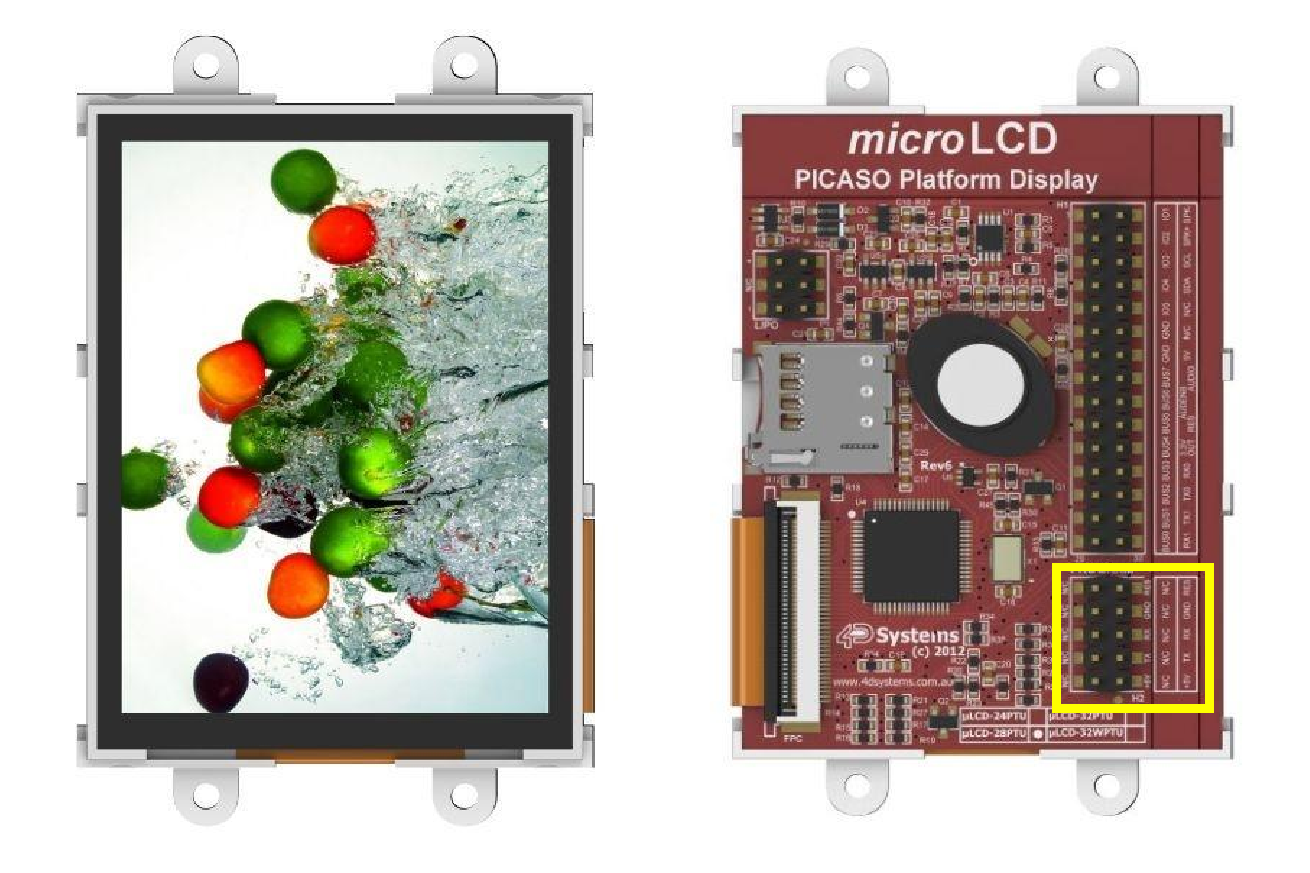
\includegraphics[scale=0.7]{ulcd-28ptu.eps}
    \caption{Display:ULCD-28PTU}
    \label{fig_ulcd}
\end{figure}

\begin{figure}
	\centering
	\scalebox{0.7}{\input{./fig/convLcdConn.pstex_t}}
	\caption{Connection diagram for USB to Serial Converter and Display}
	\label{fig_convLcdCon}
\end{figure}

The software can used with the USB to Serial converter only for learning purposes. To make a stand alone device the display needs to be interfaced with other stand alone systems like Raspberry Pi.

\section{Interfacing Raspberry Pi}
	Before making the complete product it is necessarry to have a setup in which the system can be programmed, debugged and analysed. This setup mainly concerns with how the Pi (which is connected to the display) can be interfaced to a computer. 

\subsection{Installing Raspbian}
	As mentioned before an OS, Raspbian, shall be installed in the SD card of the Pi to perform the required functions. Although 'bare metal' programming of Pi is possible it is a complex proceedure in addition of need of extra hardwares for programming. A forum dedicated to the bare metal programming of Pi is available \href{https://www.raspberrypi.org/forums/viewforum.php?f=72}{here}. But here we will focus on programming via the OS.

	Any image burning software can be used to burn the ISO image downloaded from the Raspbian site. A recommended software is \href{https://etcher.io/}{Etcher}. A detailed explanation on how it can be used to burn the image can be found in \href{https://www.raspberrypi.org/magpi/pi-sd-etcher/}{here} \cite{bib_etcher}.

	Once the image is burned into the SD card, make an empty file named \textit{SSH} in the SD Card in the topmost directory. Raspberry Pi version 2.0 has SSH disabled by default. We are making this change to enable it. The SD card can then be inserted to the PI and then can be powered up. If a monitor with a HDMI port and a usb keyboard are available they can be directly plugged into the pi for interactions. But as these extra items were unavailable at the time of the project the Pi is configured to program remotely by SSH.

\subsection{Connection Raspbian Pi via SSH}
	
	Placing the empty \textit{SSH} file is of utmost importance for connecting the Pi, without keyboard or monitor, to a computer. The IP address to Raspberry pi can be assigned in two ways

\subsubsection{Static IP address allocation}
	\begin{enumerate}
		\item Insert the SD card to the computer (via a card reader) running on linux. It shows all the folders in the original OS.
		\item Go the file \texttt{/etc/network/interfaces}. Replace the line \texttt{iface eth0 inet dhcp} with \texttt{iface eth0 inet static}
		\item Add the following lines after the previous step
		
			\texttt{address=<ip address> \\
					netmask=<net mask> \\
					network=<network address> \\
					broadcast=<broadcast address> \\
					gateway=<gateway address>}

		where the $'< >'$ indicates the values to be given. Make sure the computer to which the Pi is connected is also in the same subnet mask.
		\item Go the file \texttt{/etc/dhcpcd.conf} and add the following lines at the end of the file
				
			\texttt{interface <interface name eg: eth0> \\
					static ip\_address=<ip address> }
		\item Insert the SD card to the Pi and boot. Once booted up, connect Pi to computer via ethernet cable. For SSH login to the Pi, use software like \textit{putty} in windows. In linux use the ssh command (for eg: \texttt{ssh pi@<ip address>}). The default username is \texttt{pi} and the password is \texttt{raspberry}.
	\end{enumerate}	

The disadvantage of this method is that Pi will not be connected to the internet if you want to download and install any packages. So a better solution is using dynamic IP allocation.

\subsubsection{Dynamic IP allocation}
	Here WiFi connection will be shared with the ethernet port for dynamic IP allocation and making available internet to Pi.

	\begin{enumerate}
		\item After burning the image and putting an empty \textit{SSH} file, connect the SD card to Pi and connect Pi to the computer, with a WiFi connection, via ethernet cable. Here it is assumed that the file \texttt{/etc/network/interfaces} has \texttt{iface eth0 inet manual} as default setup. If there is failure of connection, then the file needed to be manualy edited to \texttt{iface eth0 inet manual} with all the IP address commented throught the steps mentioned in previous section.
		\item Make sure the Wifi is connected to some network. Share the WiFi adapter to share its internet connection with the ethernet. Make sure the IP address are kept as \textit {Obtain IP address dynamically} for both the WiFi and ethernet. The system will assign an ip address to the ethernet port and the device connected to it automatically. That is raspberry pi will be assigned an IP address.
		\item To find out what is the ip address assigned to Pi, first get the IP address of the ethernet port of the computer (this can be obtained by giving \texttt{ipconfig} command in windows). Install \texttt{nmap} from \href{https://nmap.org/download.html}{here}. If the ip address obtained for ethernet is \texttt{a.b.c.d} then given the command \texttt{nmap -sn a.b.c.0/24} in the command window. It will lists all the devices within this range connected to the ethernet port along with the name of the device.
		\item Identify the ip address of Pi and connect it via putty.
	\end{enumerate}

\textbf{The current configuration of Pi with static ip address of 192.168.137.2}

A python program will be running in the Pi which controls the display.

\section{Interfacing Raspberry Pi with ULCD-28PTU}

	The Pi is interfaced to the display via UART. The schematic of the PI can be found in the website \href{https://www.raspberrypi.org/documentation/hardware/raspberrypi/schematics/Raspberry-Pi-2B-V1.2-Schematics.pdf}{here} \cite{bib_pisch}. Only the relevant portion of the schematic is shown in fig(\ref{fig_pisch})

\begin{figure}
	\centering
	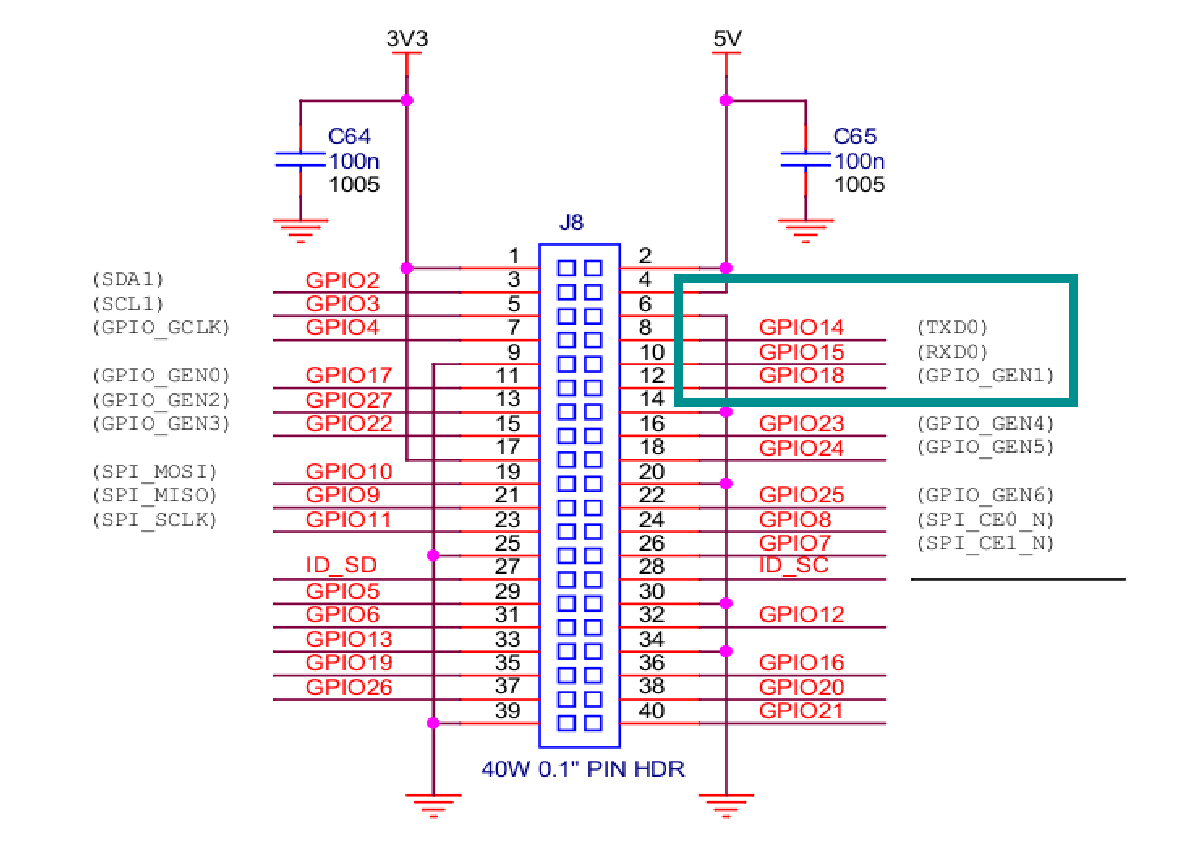
\includegraphics[scale=0.65]{./fig/rpisch.eps}
	\caption{Schematic of Raspberry Pi for connecting with the display}
	\label{fig_pisch}
\end{figure}
	
The connectors shown in cyan colored box in the fig(\ref{fig_pisch}) are connected to the connectors in yellow colored box in fig(\ref{fig_ulcd}). The fig(\ref{fig_convLcdCon}) will be the same except that the USB to serial converter block will be replaced by Pi and the \texttt{DTR} pin of the converter will be replaced by \texttt{GPIO\_GEN1} pin of the Pi for resetting purposes.

\subsection{The Code}
	Once these connections are made each and every pixel of the ULCD display can be controlled by serial commands send from the Pi. A sample program has been done in the github. The link is \href{https://github.com/jinujayachandran/dso}{here}\cite{bib_code}. The \texttt{dso.py} file have the latest code of displaying two sine waves simultaneously in the display. The comments of the code gives information of the algorithm used. After proper connections are made run the code for the display.

\section{What's Next?}
	The system can be improved as follows
\begin{enumerate}
	\item Improving the current algorithm. The current algorithm has some amount of delay in showing one waveform after the other. The main reason is because the screen is cleared after displaying one complete wave. The algorithm can be improved so that we will observe a standing wave. The logic of trigger functionality of the practical DSO's can be made use for the same. 
	\item Interfacing of external ADC to Pi via SPI or I2C.
	\item Accumulate, Process and Display the values obtained from ADC. The current code can be modified in such a way that instead of generating sine values, the values can shall be obtained from ADC, convert it to voltage and scale the values to display on display.
	\item Finding the parameters of the wave such as frequency, peak voltage, average voltage etc and displaying them are not yet explored. 
	\item The ULCD-28PTU display is also a touch screen. There are serial commands which allows to get the values of pixel when touched. This is can be used to make it more user friendly. For example by scrolling the screen increases resolution of the signal displayed.
\end{enumerate}

\bibliographystyle{plain}
\bibliography{dso}
 
\end{document}


